\section{Data Release Production}
\label{sec:drp}

\begin{figure}
\centering
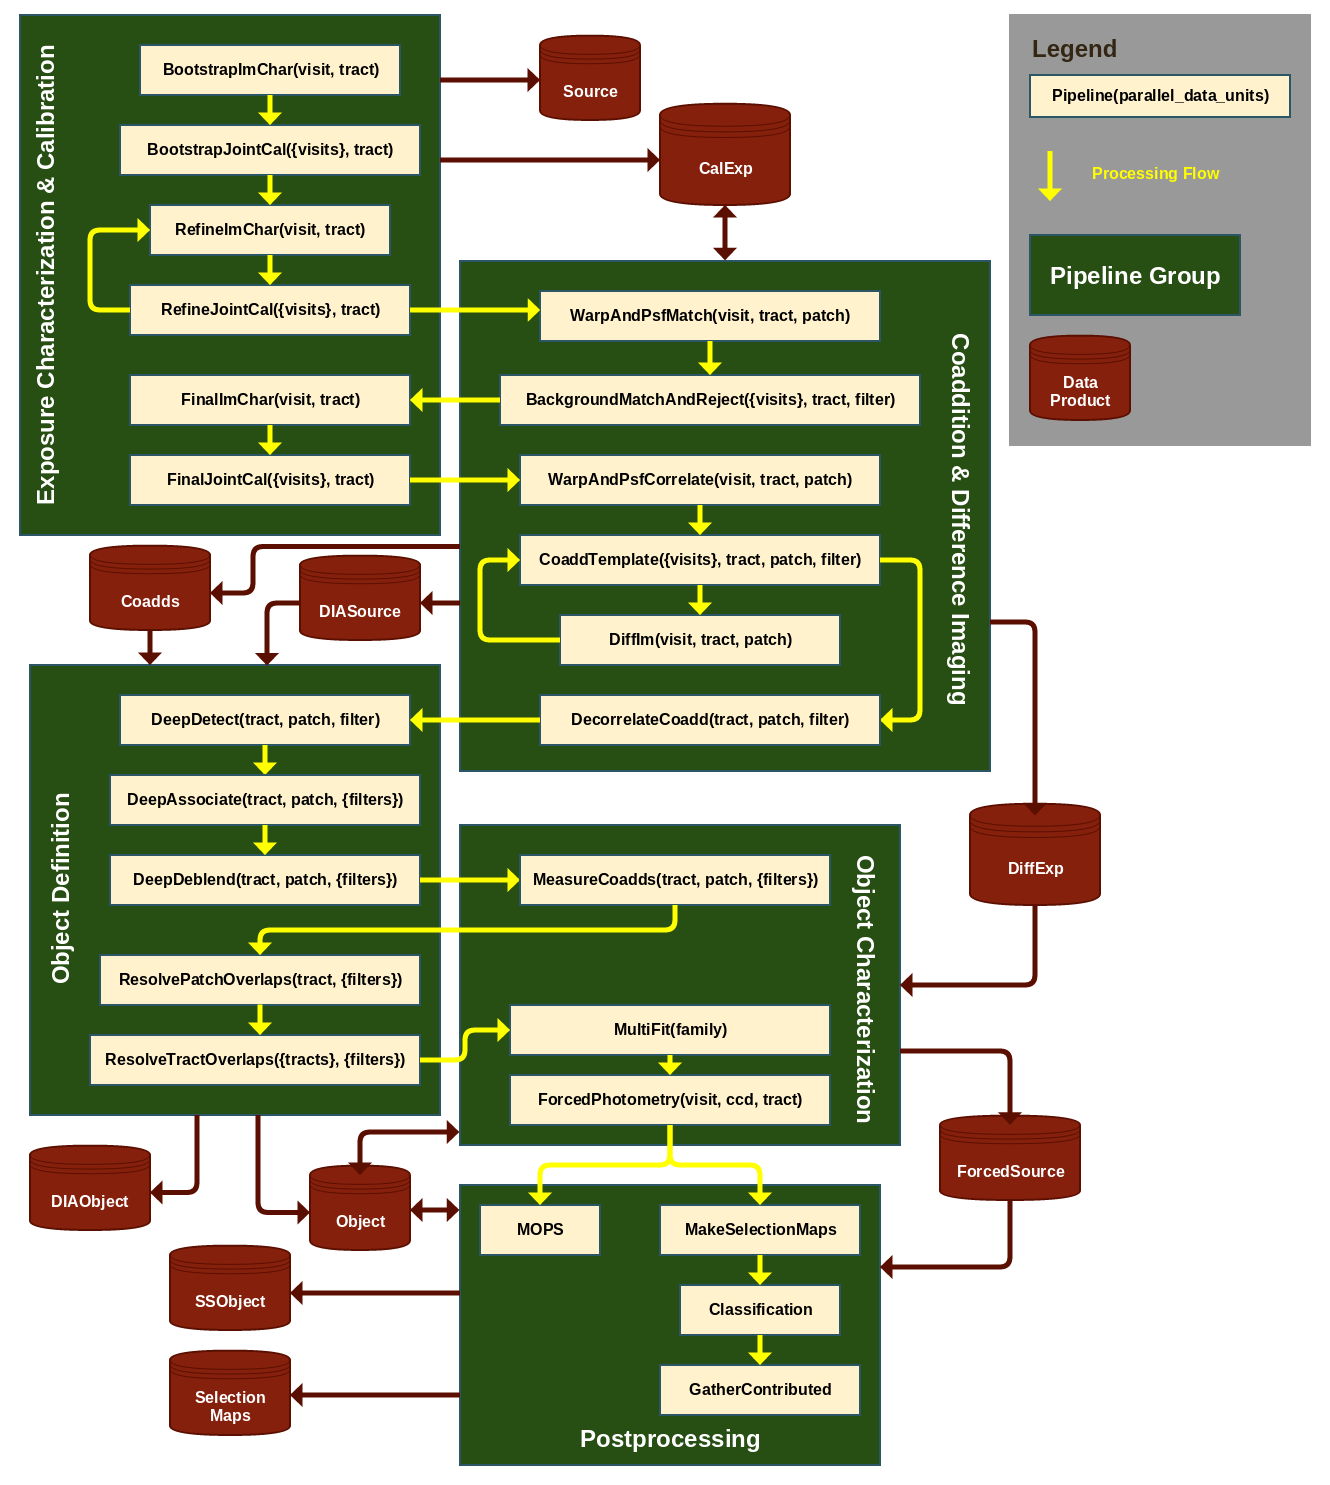
\includegraphics[width=\textwidth]{figures/drp_summary.png}
\caption{Summary of the Data Release Production processing flow.  Processing is split into multiple pipelines, which are conceptually organized into the groups discussed in sections~\ref{sec:drp_imchar_and_jointcal}-\ref{sec:drp_postprocessing}.
\label{fig:drp_summary}}
\end{figure}

A Data Release Production is run every year (twice in the first year of operations) to produce a set of catalog and image data products derived from all observations from the beginning of the survey to the point the production began.  This includes running a variant of the difference image analysis run in Alert Production, in addition to direct analysis of individual exposures and coadded images.  The data products produced by a Data Release Production are summarized in table~\ref{table:drp_data_products}.


\begin{table}
\small
\begin{tabularx}{\textwidth}{ | l | l | X | }
  \hline
  {\bf Name} & {\bf Availability} & {\bf Description} \\
  \hline
  Source & Stored &
  Measurements from direct analysis of individual exposures. \\
  \hline
  DIASource & Stored &
  Measurements from difference imagine analysis of individual exposures. \\
  \hline
  Object & Stored &
  Measurements for a single astrophysical object, derived from all available information, including coadd measurements, simultaneous multi-epoch fitting, and forced photometry.  Does not include solar system objects. \\
  \hline
  DIAObject& Stored &
  Aggregate quantities computing by associating spatially colocated DIASources. \\
  \hline
  ForcedSource & Stored &
  Flux measurements on each direct and difference image at the position of every Object. \\
  \hline
  SSObject & Stored &
  Solar system objects derived by associating DIASources and inferring their orbits. \\
  \hline
  CalExp & Regenerated &
  Calibrated exposure images for each CCD/visit (sum of two snaps). \\
  \hline
  DiffExp & Regenerated &
  Difference between CalExp and PSF-matched template coadd. \\
  \hline
  DeepCoadd & Stored &
  Coadd image with a reasonable combination of depth and resolution. \\
  \hline
  EpochRangeCoadd & Renegerated &
  Coadd image that cover only a limited range of epochs. \\
  \hline
  BestSeeingCoadd & Regenerated &
  Coadd image built from only the best-seeing images. \\
  \hline
  PSFMatchedCoadd & Regenerated &
  Coadd image with a constant, predetermined PSF. \\
  \hline
\end{tabularx}
\caption{Table of public data products produced during a Data Release Production.  A full description of these data products can be found in the Data Products Definition Document (LSE-163).
\label{table:drp_data_products}}
\end{table}

From a conceptual standpoint, data release production can be split into five groups of pipelines, executed in approximately the following order:
\begin{enumerate}
\item We characterize and calibrate each exposure, estimating point-spread functions, background models, and astrometric and photometric calibration solutions.  This iterates between processing individual exposures independently and jointly fitting catalogs derived from multiple overlapping exposures.  These steps are described more fully in section~\ref{sec:drp_imchar_and_jointcal}.
\item We alternately combine images and subtract them, using differences to find artifacts and time-variable sources while building coadds that produce a deeper view of the static sky.  Coaddition and difference imaging is described in section~\ref{sec:drp_coaddition_and_diffim}.
\item We detect and deblend on coadds, while associating these detection with detections from difference imaging to define objects.  We then merge catalogs in the overlap regions between patches and tracts to produce a single contiguous catalog over the full sky.  This is described in section~\ref{sec:drp_object_definition}.
\item We measure objects on coadds and visit-level direct and difference images in object characterization, as described section~\ref{sec:drp_object_characterization}.
\item After all image processing is complete, we run additional catalog-only pipelines to fill in additional object properties.  Unlike previous stages, this postprocessing is not localized on the sky, as it may use statistics computed from the full data release to improve our characterization of individual objects.  Postprocessing pipelines are described in section~\ref{sec:drp_postprocessing}.
\end{enumerate}
This conceptual ordering is an oversimplification of the actual processing flow, however; as shown in Figure~\ref{fig:drp_summary}, pipeline groups are actually interleaved.

Each pipeline in this the diagram represents a particular piece of code excuted in parallel on a specific unit of data, but pipelines may contain additional (and more complex) parallelization to further subdivide that data unit.  The processing flow also includes the possibility of iteration between pipelines, indicated by cycles in the diagram.  The number of iterations in each cycle will be determined (via tests on smaller productions) before the start of the production, allowing us to remove these cycles simply by duplicating some pipelines a fixed number of times.  The final data release production processing can thus be described as a directed acyclic graph (DAG) to be executed by the orchestration middleware, with pipelines as edges and (intermediate) data products as vertices.  Most of the graph will be generated by applications code before the production begins, using a format and/or API defined by the orchestration middleware.  Howver, some parts of the graph must be generated on-the-fly; this will be discussed further in section~\ref{sec:drpMultiFit}.


\subsection{Image Characterization and Calibration}
\label{sec:drp_imchar_and_jointcal}

\begin{note}[ImChar/JointCal Diagram]
Extract ImChar/JointCal pipelines from ``DRP Top-Level Overview'' on confluence and expand detail to show data flow and ordering of ``Task/Process'' boxes.
\end{note}

The first steps in a Data Release Production characterize the properties of individual exposures, by iterating between pixel-level processing of individual visits (``ImChar'', or ``Image Characterization'' steps) and joint fitting of all catalogs overlapping a tract (``JointCal'', or ``Joint Calibration'' steps).  All ImChar steps involve fitting the PSF model and measuring Sources (gradually improving these as we iterate), while JointCal steps fit for new astrometric (WCS) and photometric solutions while building new reference catalogs for the ImChar steps.  Iteration is necessary for a few reasons:
\begin{itemize}
\item The PSF and WCS must have a consistent definition of object centroids.  Celestial positions from a reference catalog are transformed via the WCS to set the positions of stars used to build the PSF model, but the PSF model is then used to measure debiased centroids that feed the WCS fitting.
\item The later stages of photometric calibration and PSF modeling require secure star selection and colors to infer their SEDs.  Magnitude and morphological measurements from ImChar stages are aggregated the reference catalog in the subsequent JointCal stage, allowing these colors and classifications to be used for PSF modeling in the following ImChar stage.
\end{itemize}

The ImChar and JointCal iteration is itself interleaved with background matching, described in section~\ref{sec:drp_coaddition_and_diffim}.  This allows the best backgrounds and masks to be defined in the \hyperref[drpBackgroundMatchAndReject]{BackgroundMatchAndReject} before the final Source measurements, image characterizations, and calibrations.

Each ImChar pipeline runs on a single visit, and each JointCal pipeline runs simultaneously on all visits within a single tract, allowing tracts to be run entirely independently.

The final output data products of the ImChar/JointCal iteration are the Source table and CalExp (calibrated exposure) images.  The latter includes Image, Mask, Variance, Background, PSF, WCS, Calib components that we will track separately.

There are also several intermediate versions of the Source and CalExp data products passed between the ImChar/JointCal pipelines, as well as...

\subsubsection{BootstrapImChar}
\label{sec:drpBootstrapImChar}

The BootstrapImChar pipeline is the first thing run on each science exposure in a data release.  It has the difficult task of bootstrapping multiple quantities (PSF, WCS, photometric calibration, background model, etc.) that each normally require all of the others to be specified when one is fit.  As a result, while the algorithmic components to be run in this pipeline are generally clear, their ordering and specific requirements are not; algorithms that are run early will have a harder task than algorithms that are run later, and some iteration will almost certainly be necessary.

A plausible (but by no means certain) high-level algorithm for this pipeline is given below in pseudocode.  Highlighted terms are described in more detail below the pseudocode block.

\lstset{
    language=Python,
    basicstyle=\scriptsize\ttfamily,
    keywordstyle=\bfseries,
    commentstyle=\color{darkgray},
    escapeinside={\%}{\%},
}

% Define a local macro that lets us refer to sections of the text
% more easily (will undefine at the end of this section).
\newcommand{\hr}[1]{\hyperref[sec:drpBootstrapImChar_#1]{#1}}

\begin{lstlisting}
def BootstrapImChar(%\hr{raw}%, %\hr{reference}%):
    # Some data products components are visit-wide and some are per-CCD;
    # these imaginary data types lets us deal with both.
    # VisitExposure also has components; most are self-explanatory, and
    # {mi} == {image,mask,variance} (for "MaskedImage").
    calexp = VisitExposure()
    sources = VisitCatalog()
    parallel for ccd in ALL_SENSORS:
        snaps = [%\hr{RunISR}%(raw[ccd]) for snap in raw]
        calexp[ccd].mask = %\hr{FindArtifacts}%(snaps[ccd])
        calexp[ccd].{mi} = %\hr{CombineSnaps}%(calexp[ccd].mask, snaps)
    calexp.psf = %\hr{FitWavefront}%(calexp[WAVEFRONT_SENSORS].mi)
    calexp.{image,mask,variance,background}
        = %\hr{SubtractBackground}%(calexp.mi)
    parallel for ccd in SCIENCE_SENSORS:
        sources[ccd] = %\hr{DetectSources}%(calexp.{mi,psf})
    matches = %\hr{MatchSemiBlind}%(sources, reference)
    while not converged:
        %\hr{SelectStars}%(matches, exposures)
        calexp.wcs = %\hr{FitWCS}%(matches, sources, reference)
        calexp.psf = %\hr{FitPSF}%(matches, sources, calexp.{mi,wcs})
        %\hr{WriteDiagnostics}%(calexp, sources)
        parallel for ccd in SCIENCE_SENSORS:
            calexp[ccd].mask = %\hr{FindArtifacts}%(calexp[ccd].{mi,psf})
            calexp[ccd].{mi} = %\hr{InterpolateArtifacts}%(calexp[ccd].{mi,psf})
            calexp[ccd].{mi} = %\hr{SubtractStars}%(calexp[ccd].{mi,psf}, sources[ccd])
        calexp.{mi,background} = %\hr{SubtractBackground}%(calexp.mi)
        parallel for ccd in SCIENCE_SENSORS:
            sources[ccd] = %\hr{DetectSources}%(calexp.{mi,psf})
            sources[ccd] = %\hr{DeblendSources}%(sources[ccd], calexp.{mi,psf})
            sources[ccd] = %\hr{MeasureSources}%(sources[ccd], calexp.{mi,psf})
        matches = %\hr{MatchNonBlind}%(sources, reference)
    calexp.psf.apcorr = %\hr{FitApCorr}%(matches, sources)
    parallel for ccd in SCIENCE_SENSORS:
        sources[ccd] = %\hr{ApplyApCorr}%(sources[ccd], calexp.psf)
    calexp.calib = %\hr{FitPhotoCalib}%(matches, sources)
    return calexp, sources
\end{lstlisting}

\paragraph{Input Data Product: Raw}
\label{sec:drpBootstrapImChar_raw}
Raw amplifier images from science and wavefront CCDs, spread across one or more snaps.  Needed telescope telemetry (seeing estimate, approximate pointing) is assumed to be included in the raw image metadata.

\paragraph{Input Data Product: Reference}:
\label{sec:drpBootstrapImChar_reference}
A full-sky catalog of reference stars derived from both external (e.g. Gaia) and LSST data.

Later pipelines (\hyperref[sec:drpBootstrapJointCal]{BootstrapJointCal}, \hyperref[sec:drpRefineJointCal]{RefineJointCal}) will define a deeper reference catalog derived from this one and the new data being processed, but the origin and depth of the initial reference catalog is largely TBD.  It will almost certainly include Gaia stars, but it may also include data from other telescopes, LSST special programs, LSST commissioning observations, and/or the last LSST data release.

\paragraph{Output Data Product: Source.}
\label{sec:drpBootstrapImChar_sources}

A preliminary version of the Source table.  This could contain all of the columns in the DPDD Source schema if the \hr{MeasureSources} is appropriately configured, but some of these columns are likely unnecessary in its role as an intermediate data product that feeds \hyperref[sec:drpBootstrapJointCal]{BootstrapJointCal}, and it is likely that other non-DPDD columns will be present for that role.

BootstrapImChar also has the capability to produce even earlier versions of the Source table for diagnostic purposes (see \hr{writeDiagnostics}).  These tables are not associated with any photometric calibration or aperture correction, and some may not have any measurements besides centroids, and hence are never substitutable for the final Source table.

\paragraph{Output Data Product: CalExp}
\label{sec:drpBootstrapImChar_calexp}

A preliminary version of the CalExp (calibrated direct exposure).  CalExp is an \hyperref[sec:spImagesExposure]{Exposure} object, and hence it has several components.  BootstrapImChar is the only pipeline that actually updates all of them.  Some CalExp components are determined at the scale of a full FoV and hence should probably be persisted at the visit level (PSF, WCS, Calib, Background), while others are straightforward CCD-level data products (Image, Mask, Variance).

\paragraph{RunISR}
\label{sec:drpBootstrapImChar_RunISR}

\paragraph{FindArtifacts}
\label{sec:drpBootstrapImChar_FindArtifacts}

\paragraph{CombineSnaps}
\label{sec:drpBootstrapImChar_CombineSnaps}

\paragraph{InterpolateArtifacts}
\label{sec:drpBootstrapImChar_InterpolateArtifacts}

\paragraph{FitWavefront}
\label{sec:drpBootstrapImChar_FitWavefront}

\paragraph{SubtractBackground}
\label{sec:drpBootstrapImChar_SubtractBackground}

\paragraph{DetectSources}
\label{sec:drpBootstrapImChar_DetectSources}

\paragraph{MatchSemiBlind}
\label{sec:drpBootstrapImChar_MatchSemiBlind}

\paragraph{FitWCS}
\label{sec:drpBootstrapImChar_FitWCS}

\paragraph{FitPSF}
\label{sec:drpBootstrapImChar_FitPSF}

\paragraph{WriteDiagnostics}
\label{sec:drpBootstrapImChar_WriteDiagnostics}

\paragraph{SubtractStars}
\label{sec:drpBootstrapImChar_SubtractStars}

\paragraph{DeblendSources}
\label{sec:drpBootstrapImChar_DeblendSources}

\paragraph{MeasureSources}
\label{sec:drpBootstrapImChar_MeasureSources}

\paragraph{MatchNonBlind}
\label{sec:drpBootstrapImChar_MatchNonBlind}

\paragraph{FitApCorr}
\label{sec:drpBootstrapImChar_FitApCorr}

\paragraph{ApplyApCorr}
\label{sec:drpBootstrapImChar_ApplyApCorr}

\paragraph{FitPhotoCalib}
\label{sec:drpBootstrapImChar_FitPhotoCalib}

% Undeclare the local hyperref macro
\let\hr\undefined

\begin{itemize}
\item \hyperref[sec:acISR]{ISR}
  \begin{itemize}
  \item On snaps
  \item Includes all the B-F correction we need.
  \item Flat field image to color of sky?
  \end{itemize}
\item \hyperref[sec:acSnapSubtraction]{Subtract} and \hyperref[sec:acCoaddition]{Combine} Snaps.
  \begin{itemize}
  \item If we don't take two snaps, do \hyperref[sec:acMorphogicalArtifactDetection]{morphological artifact detection} instead.
  \item If combining/diffing snaps requires warping, this is \emph{much} harder, to the point that we should only take one snap.
  \end{itemize}
\item \hyperref[sec:acBackgroundEstimation]{background estimation}
  \begin{itemize}
  \item Only need to detect and measure bright stars, so aggresive background subtraction is okay and possibly desirable.
  \item Need to ensure flat-fielding and pixel area corrections are appropriate for background estimation at this point.
  \item In crowded fields, we want to initially subtract most faint stars, leaving only bright ones.
  \end{itemize}
\item \hyperref[sec:acSourceDetection]{source detection}.
  \begin{itemize}
  \item In crowded fields detect brightest stars
  \end{itemize}
\item \hyperref[sec:SingleVisitMeasurement]{Measurement}.
  \begin{itemize}
  \item Only need centroiders, shapes, aperture fluxes
  \item Needs to run w/o PSF model, or PSF guess.
  \end{itemize}
\item \hyperref[sec:acPSFStarSelection]{Select stars for PSF modeling}
  \begin{itemize}
  \item Only need centroiders, shapes, aperture fluxes
  \item Needs to run w/o PSF model, or PSF guess.
  \end{itemize}
\item \hyperref[sec:acSingleCCDPSF]{Initial PSF Modeling}
\end{itemize}

\subsubsection{BootstrapJointCal}
\label{sec:drpBootstrapJointCal}
\subsubsection{RefineImChar}
\label{sec:drpRefineImChar}
\subsubsection{RefineJointCal}
\label{sec:drpRefineJointCal}
\subsubsection{FinalImChar}
\label{sec:drpFinalImChar}
\subsubsection{FinalJointCal}
\label{sec:drpFinalJointCal}

\subsection{Coaddition and Difference Imaging}
\label{sec:drp_coaddition_and_diffim}

\begin{note}[Coaddition, DiffIm Diagram]
Extract Coaddition and DiffIm pipelines from ``DRP Top-Level Overview'' on confluence and expand detail to show data flow and ordering of ``Task/Process'' boxes.
\end{note}

\subsubsection{WarpAndPsfMatch}
\label{sec:drpWarpAndPsfMatch}
\subsubsection{BackgroundMatchAndReject}
\label{sec:drpBackgroundMatchAndReject}
\subsubsection{WarpAndPsfCorrelate}
\label{sec:drpWarpAndPsfCorrelate}
\subsubsection{CoaddTemplate}
\label{sec:drpCoaddTemplate}
\subsubsection{DiffIm}
\label{sec:drpDiffIm}
\subsubsection{DecorrelateCoadds}
\label{sec:drpDecorrelateCoadds}

\subsection{Object Definition}
\label{sec:drp_object_definition}

\begin{note}[Detection/Association/Deblending Diagram]
Extract process\_coadds pipeline from ``DRP Top-Level Overview'' on confluence and expand detail to show data flow and ordering of ``Task/Process'' boxes.
\end{note}

\subsubsection{DeepDetect}
\label{sec:drpDeepDetect}
\subsubsection{DeepAssociate}
\label{sec:drpDeepAssociate}
\subsubsection{DeepDeblend}
\label{sec:drpDeepDeblend}
\subsubsection{ResolvePatchOverlaps}
\label{sec:drpResolvePatchOverlaps}
\subsubsection{ResolveTractOverlaps}
\label{sec:drpResolveTractOverlaps}

\subsection{Object Characterization}
\label{sec:drp_object_characterization}

\begin{note}[Object Characterization Diagram]
Extract multifit/forced\_photometry pipelines from ``DRP Top-Level Overview'' on confluence and expand detail to show data flow and ordering of ``Task/Process'' boxes.
\end{note}

\subsubsection{MeasureCoadds}
\label{sec:drpMeasureCoadds}
\subsubsection{MultiFit}
\label{sec:drpMultiFit}
\subsubsection{ForcedPhotometry}
\label{sec:drpForcedPhotometry}

\subsection{Postprocessing}
\label{sec:drp_postprocessing}

\begin{note}[Postprocessing Diagram]
Extract Afterburner pipelines from ``DRP Top-Level Overview'' on confluence and expand detail to show data flow and ordering of ``Task/Process'' boxes.
\end{note}

\subsubsection{MOPS}
\label{sec:drpMOPS}
\subsubsection{MakeSelectionMaps}
\label{sec:drpMakeSelectionMaps}
\subsubsection{Classification}
\label{sec:drpClassification}
\subsubsection{GatherContributed}
\label{sec:drpGatherContributed}
